\documentclass[10pt]{article}
\usepackage{graphicx} % Required for including images
\usepackage[T1]{fontenc} % Use 8-bit encoding that has 256 glyphs
\usepackage[utf8]{inputenc} % Required for including letters with accents
\usepackage[german]{babel} % Since we write our text in German
\usepackage{amsmath,amssymb,amsthm} % For including math equations, theorems, symbols, etc
\usepackage{quotes} % for quotation marks
\usepackage{caption}
\usepackage[table]{xcolor}
\captionsetup{font=footnotesize}

\title{Fachartikel}

\begin{document}

\begin{titlepage}

\raggedleft % Right align everything
	
	\vspace*{\baselineskip} % Whitespace at the top of the page
	
	\rightline{{\large Claudio Frei, Karin Birle, Leo Rudin,}} 
	\rightline{\large Michael Wigger, Nathalie Achtnich, Philippe Schneider,} 
	\rightline{\large Raphael Krebs, Silvan Nigg, Stefan Enz}
	
	\vspace*{0.167\textheight} % Whitespace before the title
	
	\textbf{\LARGE Virtual CT Board}\\[\baselineskip] % First title line
	
	\Huge Fachartikel\\[\baselineskip] % Main title line 
	
	\vfill % Whitespace 
	
	{\large ZHAW SoE - FS 2022}
	
	\vspace*{3\baselineskip} % Whitespace at the bottom of the page


\end{titlepage}

\section*{Abstract}
\thispagestyle{empty}

% Einleitung
% Methodische Einordnung der Arbeit
% Vorgehen
% Ergebnis

Ein fester Bestandteil des Informatikstudiums an der ZHAW ist das Modul \glqq Computertechnik 1\grqq, in dem die Studierenden das hardwarenahe Programmieren erlernen. Dafür wird ihnen ein physisches Microcontroller-Board zur Verfügung gestellt, das für die Durchführung der zum Modul gehörigen Praktika notwendig ist. Das Projekt \glqq Virtual CT Board\grqq{} strebt die Virtualisierung dieses physischen Boards an, um den Studierenden eine handliche, digitale Version davon zur Verfügung zu stellen. Dazu wurde eine Software gebaut, die als Web-Applikation funktioniert und in einem Browser verwendbar ist. Das Projekt hatte zum Ziel, so viele Funktionen des physischen CT Boards umzusetzen, wie während der festgesetzten Projektdauer möglich wären, wobei im Zwei-Wochen-Rhythmus Reviews und Plannings gemäss der agilen SCRUM-Methode abgehalten wurden. Nachdem die Grundarchitektur erstellt war, wurden darauf aufbauend die einzelnen Funktionen des Boards und des dazugehörigen Code-Editors umgesetzt. Im Zentrum standen dabei die Lauffähigkeit von Assembly-Code und die diversen Input-/Output-Möglichkeiten des Boards.
\newline Das vorliegend umgesetzte \glqq Virtual CT Board\grqq{} ist ein Prototyp, der noch der einen oder anderen Ergänzung bedarf, bevor er das physische CT Board vollständig ersetzen kann. Der Grundstein ist jedoch gelegt: X der 14 CT1-Praktika können bereits mit dem \glqq Virtual CT Board\grqq{} durchgeführt werden. 


\newpage

\tableofcontents
\thispagestyle{empty}

\newpage 

\pagestyle{headings}

\section{Einleitung}

\subsection{Die Idee}

Jedes Jahr beginnen fast 200 Studentinnen und Studenten ein Bachelorstudium der Informatik an der ZHAW. Zu ihren Pflichtmodulen in den ersten Jahren gehört die Veranstaltung \glqq Computertechnik 1\grqq (nachfolgend CT1 genannt), die die grundlegende Funktionsweise eines Computers an der Schnittstelle zwischen Hard- und Software behandelt. Im dazugehörigen Praktikum probieren die Studierenden das erworbene Wissen selbst aus und benutzen dabei als Hardware ein Microcontroller-Board, kurz CT Board, das über einen Prozessor und einen Speicher verfügt und diverse Input-/Output-Möglichkeiten bereitstellt (siehe Abbildung \ref{ctboard}). Das CT Board wird mit einem Kabel an den Computer angeschlossen und so mit der zugehörigen Software verbunden, die Befehle an das Board übermitteln kann. Damit sie die Übungen auch zuhause durchführen können, leihen die Studierenden zu Beginn des Semesters ein solches CT Board von der Hochschule aus. Dieses muss von ihnen nach Hause transportiert und am Ende des Jahres wieder zurückgebracht werden.

\begin{figure}[h]
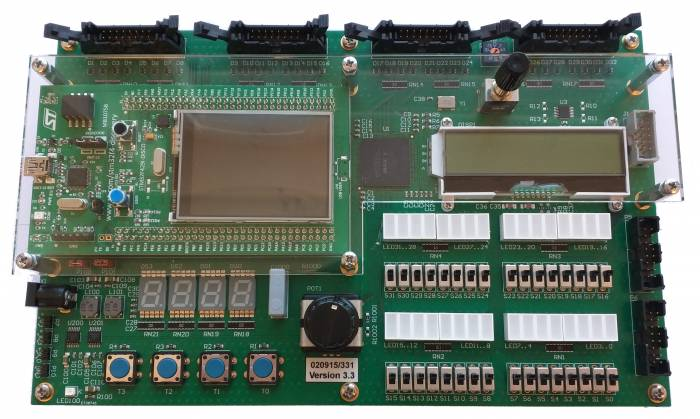
\includegraphics[width=10cm]{ctboard}
\centering
\caption{Das CT Board, das den Studenten im CT1-Modul als Hardware zur Verfügung gestellt wird. (Quelle: ennis.zhaw.ch)}
\label{ctboard}
\end{figure}

Im 21. Jahrhundert noch Hardware an Studierende auszuleihen, mutet schon fast archaisch an. Insbesondere, wenn sich die Hardware leicht als Software simulieren liesse. Und genau hier setzt die vorliegend umgesetzte Idee an: Es wird eine Web-Applikation entwickelt, die ein CT Board simuliert und in den CT1-Praktika an dessen Stelle tritt. Die Studierenden können die Übungen mit dem leichtgewichtigen \glqq Virtual CT Board\grqq{} genauso gut wie mit dem echten Board lösen und brauchen dafür fortan keine Hardware mehr. Ausserdem wird auch die bisher für die Kommunikation mit dem physischen CT Board eingesetzte Software Keil ersetzt. Das virtuelle CT Board umfasst sowohl einen Texteditor für das Schreiben von Assembly-Programmen und eine Anzeige für Register- und Memoryinhalte (bisher Keil-Funktionen) als auch eine Abbildung des CT Boards mit allen fürs  CT1-Modul relevanten Input-/Output-Funktionen. Eine Skizze der geplanten Grafikoberfläche findet sich in Abbildung \ref{draft}.

\begin{figure}[h]
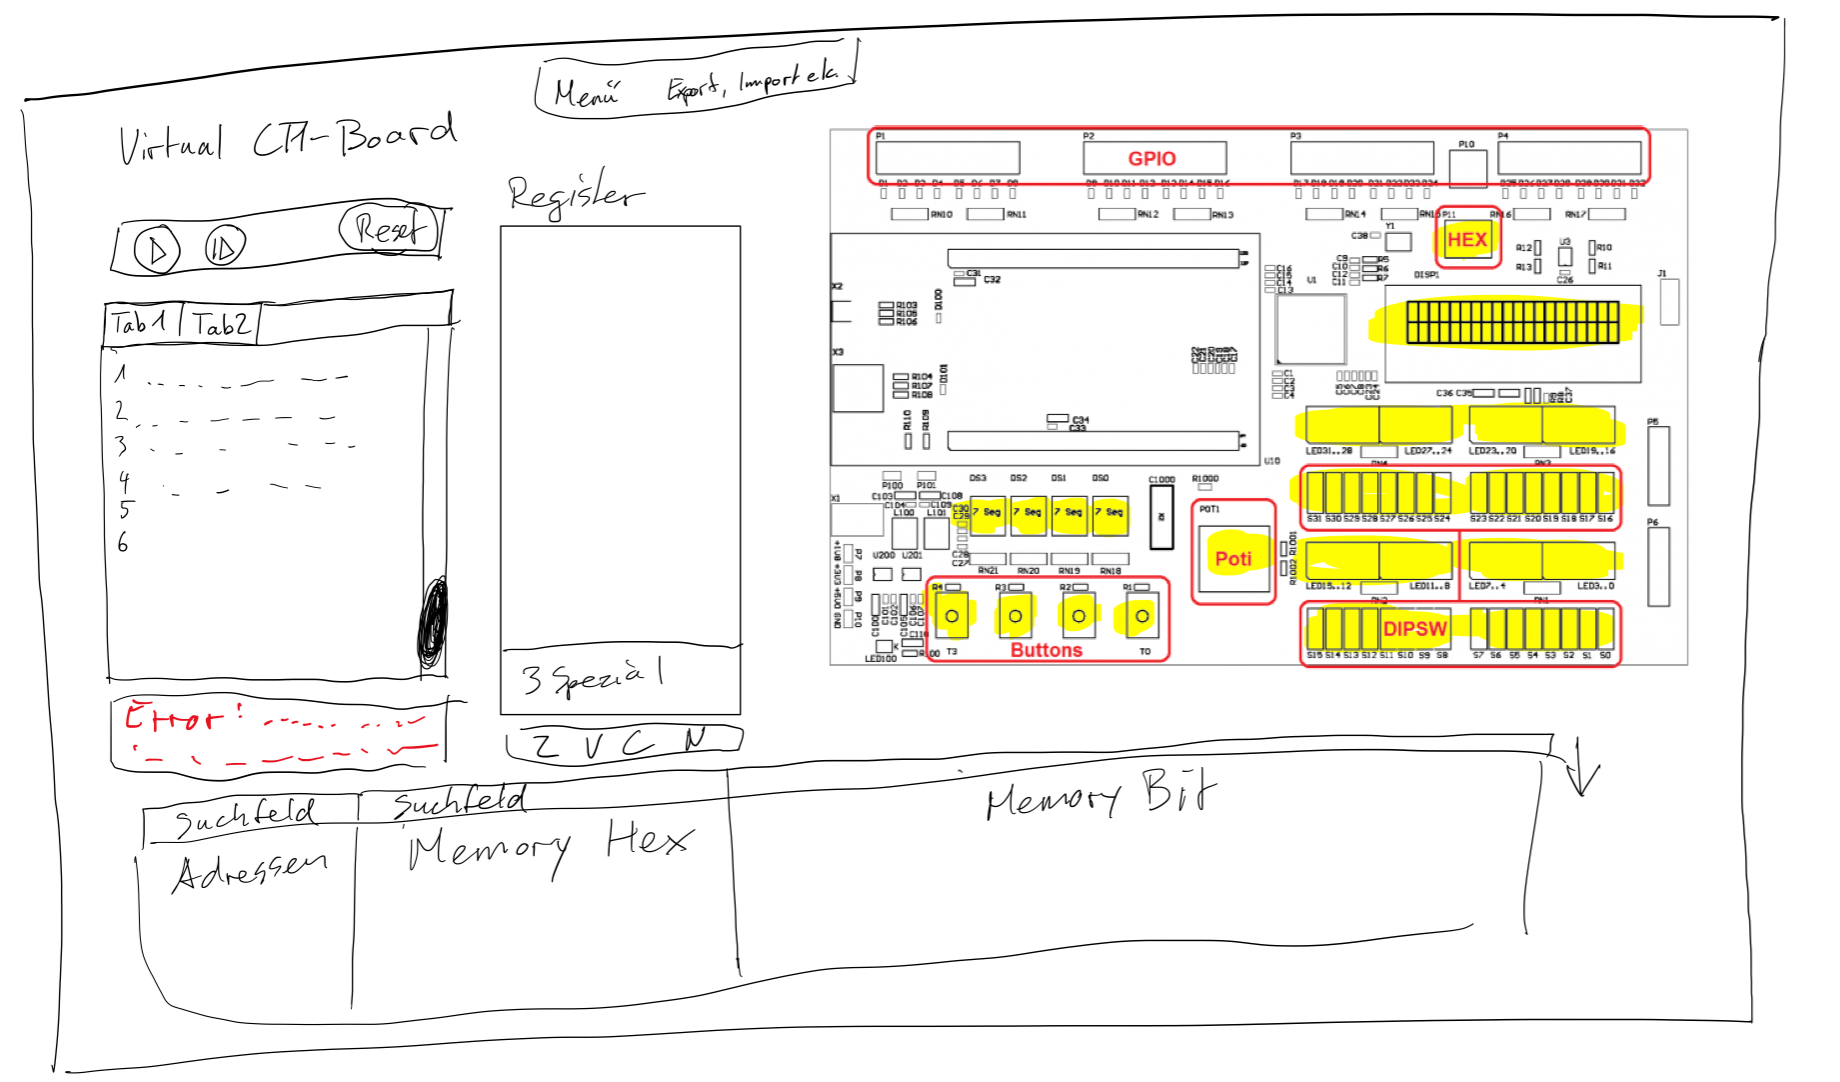
\includegraphics[width=\textwidth]{draft}
\caption[size=8pt]{Skizze der geplanten Webbrowser-Grafikoberfläche des virtuellen CT Boards.}
\label{draft}
\end{figure}

\subsection{Der Nutzen}

Zwei Zielgruppen werden als Kundschaft anvisiert, nämlich die Informatikstudierenden der ZHAW auf der einen Seite und die ZHAW als Institution auf der anderen Seite. Für beide Gruppen ergeben sich durch das vorliegend entwickelte Produkt unmittelbare Vorteile:

\paragraph{Für die Studierenden:}
\begin{itemize}
\item[$-$] Die Studierenden des CT1-Moduls haben eine elegante Alternative zu den physischen CT Boards und müssen jene nicht mehr nach Hause tragen und für ihre Erhaltung besorgt sein.
\item[$-$] Im Gegensatz zum bisherigen physischen CT Board benötigt das \glqq Virtual CT Board\grqq{} keinen Strom und lässt sich daher überall - also beispielsweise auch unterwegs - direkt auf dem Laptop starten.
\item[$-$] Alle Praktika des CT1-Moduls lassen sich mit dem \glqq Virtual CT Board\grqq{} umsetzen.
\end{itemize}

\paragraph{Für die ZHAW:}
\begin{itemize}
\item[$-$] Die Lizenz für die vorliegend entwickelte Software ist um einiges preiswerter als die Beschaffung physischer CT Boards. Ausserdem müssen alte oder defekte Geräte nicht mehr ausgetauscht oder repariert werden.
\item[$-$] Die Dozierenden müssen für die Praktika nicht mehr mühsam Keil-Projekte konfigurieren. Es genügt, die Assembler-Files ins \glqq Virtual CT Board\grqq{} hochzuladen.
\end{itemize}

\subsection{Abgrenzung zur Konkurrenz}

Es existieren bereits verschiedene Produkte, die den Studenten des CT1-Moduls beim Erlernen ihrer Fertigkeiten behilflich sein können.

\paragraph{Virtuelle Emulatoren}
Der Emulator VisUAL von Alman Sarif soll hier stellvertretend für andere virtuelle Emulatoren für die Assembly-Programmiersprache vorgestellt werden. Er wurde ebenfalls für ein Einführungsmodul in die Computerarchitektur entwickelt, allerdings am Imperial College in London. Die Software ermöglicht das Schreiben von Assembly-Code in einem Editor-Fenster, der dann via Button ausgeführt wird und dessen Auswirkungen auf die Register und Flags rechts davon angezeigt werden (siehe Abbildung \ref{emulator}).
\begin{figure}[h]
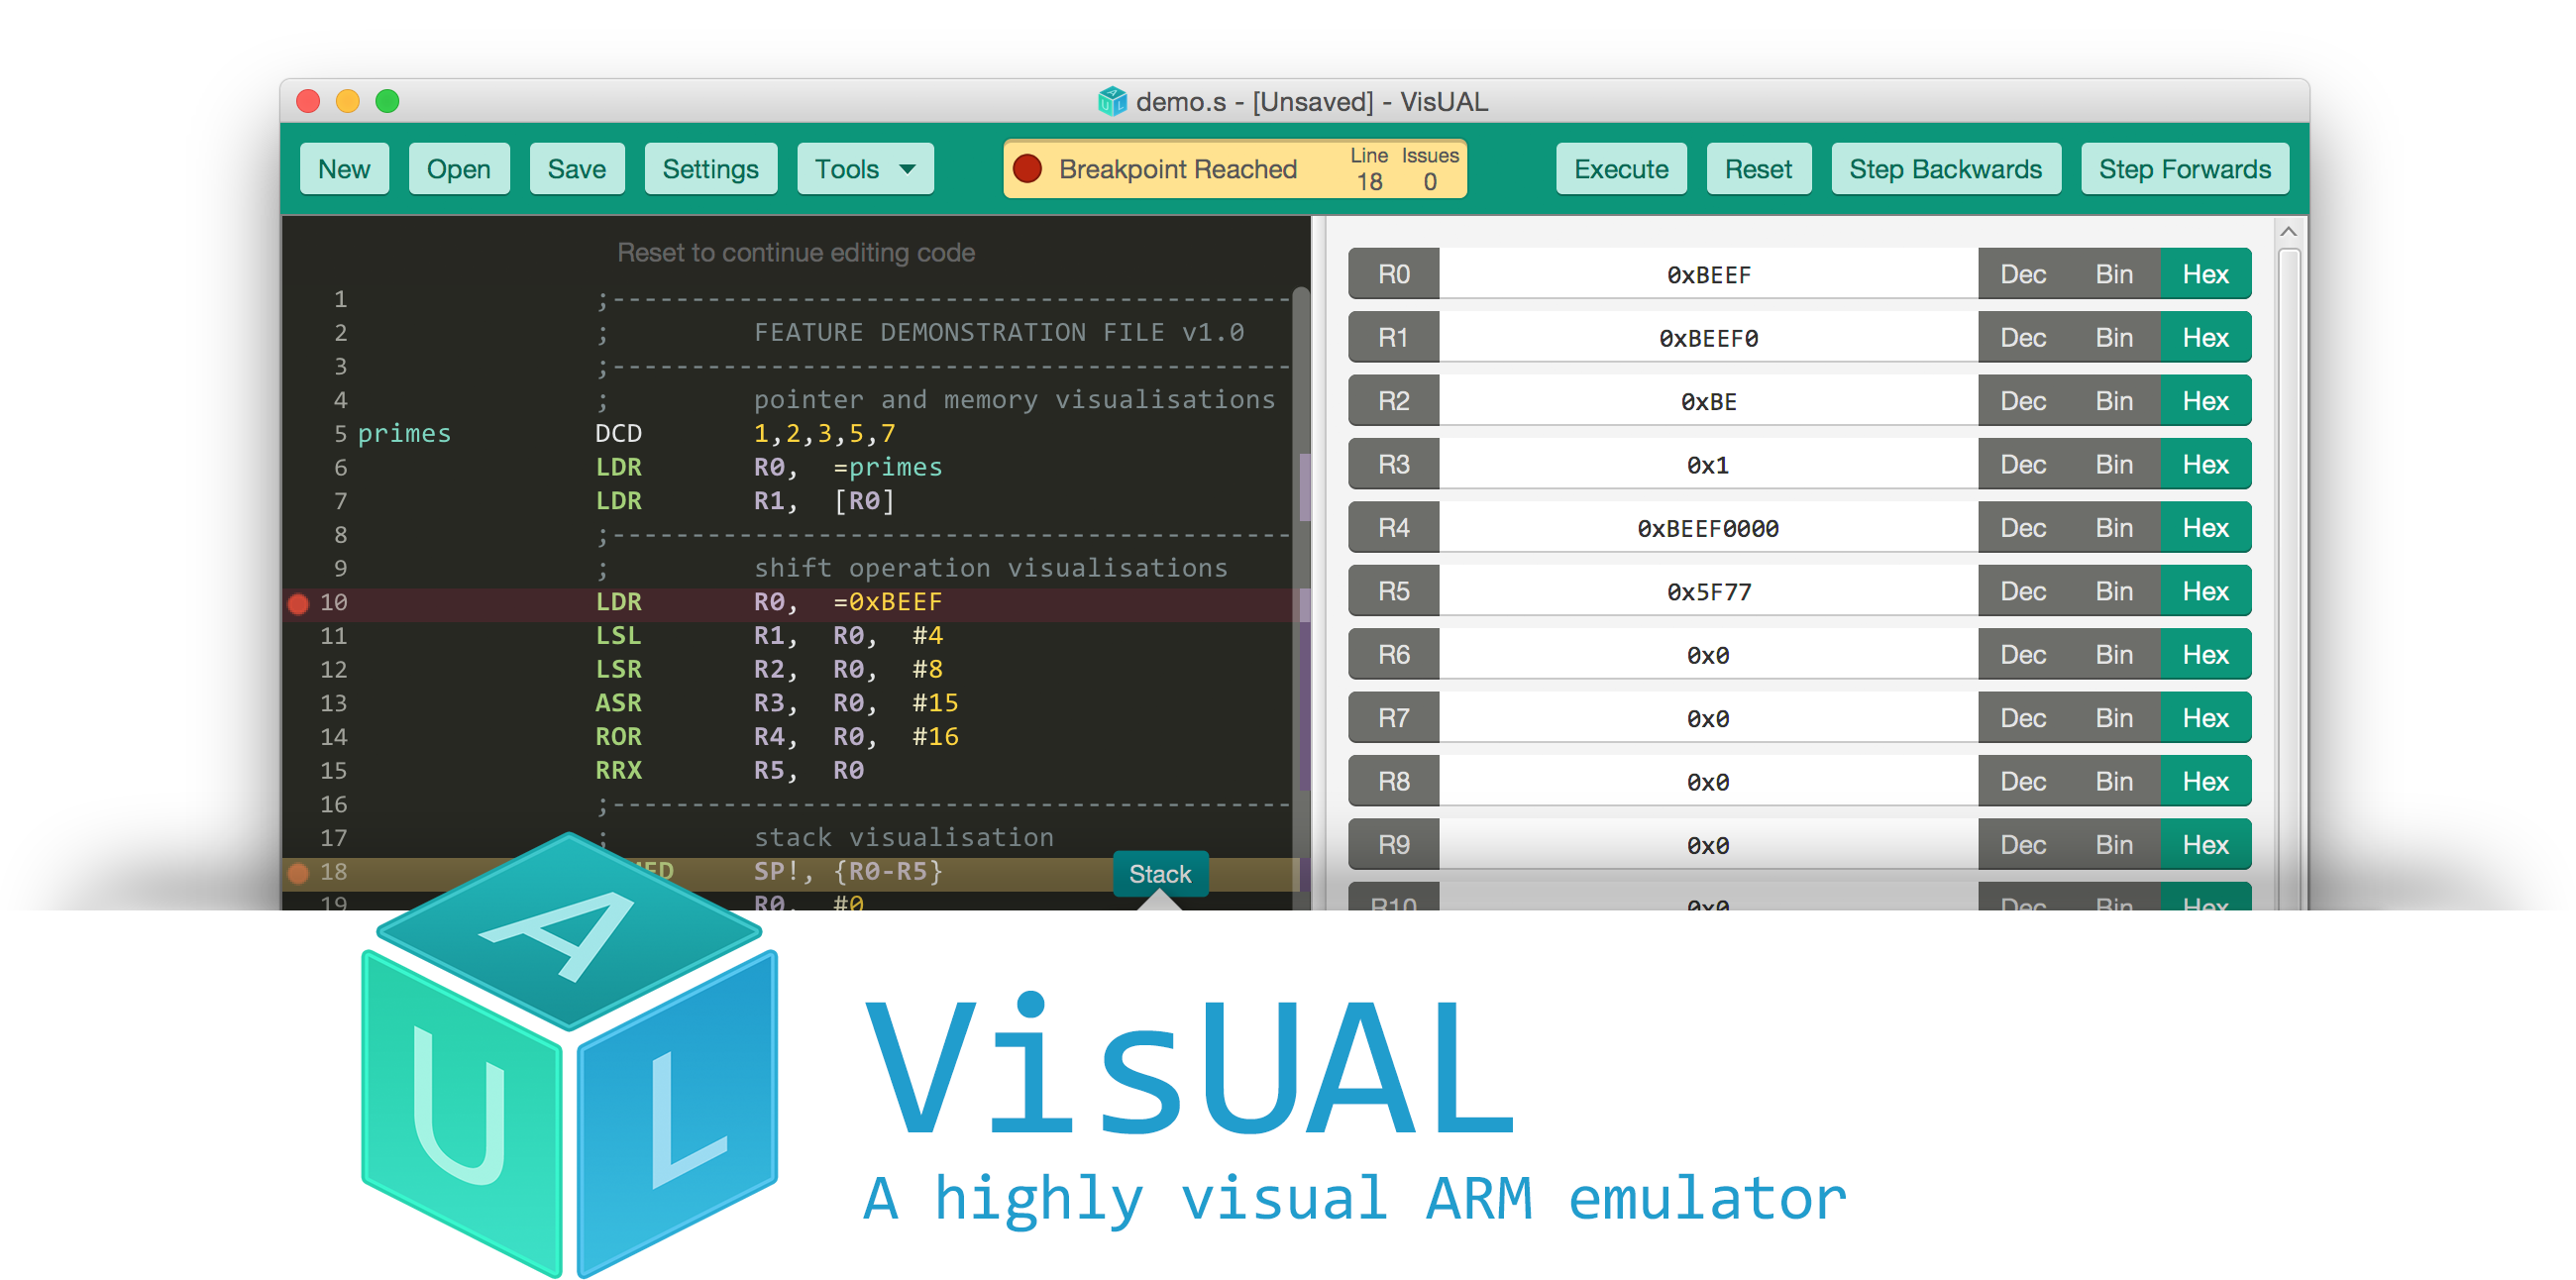
\includegraphics[width=\textwidth]{visual_emulator}
\caption{Der Emulator VisUAL samt seiner grafischen Oberfläche. (Quelle: https://salmanarif.bitbucket.io/visual/index.html)}
\label{emulator}
\end{figure}
Der Unterschied zum \glqq Virtual CT Board\grqq{} besteht darin, dass VisUAL und auch andere Assembler-Emulatoren nicht auf das CT Board ausgerichtet sind, das die CT1-Praktika verlangen. Es gibt bei diesen Programmen keine Visualisierung von Hardware-Bestandteilen, mit Ausnahme der Register und Flags. Das bedeutet, dass diese Emulatoren zwar nützlich sind, um in Assembler zu programmieren, jedoch nicht für die Durchführung der CT1-Praktika an der ZHAW ausreichen. Das \glqq Virtual CT Board\grqq{} füllt diese Lücke, indem auch die fürs CT1-Modul notwendigen Hardware-Bestandteile des physischen CT Boards visualisiert werden und dieselben Input-/Output-Möglichkeiten bestehen wie beim realen.

\paragraph{Physisches CT Board} 

Das physische CT Board soll hier noch einmal erwähnt werden, da es die Hauptkonkurrenz zum vorliegend entwickelten Produkt darstellt. Es erfüllt die funktionalen Anforderungen der CT1-Praktika vollumfänglich und ist ausserdem im Schulbetrieb bereits etabliert. Seine Nachteile bestehen insbesondere in seiner Unhandlichkeit. Das \glqq Virtual CT Board\grqq{} soll diesen Nachteil durch seine Virtualität beheben und gleichzeitig dem realen CT Board bzgl. Funktionalität in nichts nachstehen. Damit liegt es im Trend der Zeit, denn Studien belegen, dass die \emph{Digital Natives} der Generation Z den Einsatz aktueller Technologien zur Effizienzsteigerung im beruflichen Umfeld geradezu fordern (West 2018, Wirthman 2020). Somit verhilft das virtuelle CT Board dem CT1-Modul bei nachfolgenden Studentengenerationen zu neuer Attraktivität.


\subsection{Risiken}
Trotz ausführlicher und sorgfältiger technischer Analyse des Funktionsumfangs des physischen CT Boards bestehen bei dessen virtuellen Nachbau einige Risiken:
\begin{itemize}
\item[$-$] Gewisse Funktionen können virtuell nicht gleich nachgebaut werden. Insbesondere die Simulation von Interrupts könnte eine Herausforderung darstellen.
\item[$-$] Der Funktionsumfang des virtuellen Boards könnte aufgrund knapper Projektlaufzeit eingeschränkt werden. 
\item[$-$] Aufgrund falscher Implementierung können unvorhergesehene Fehler auftreten. Das virtuelle Board wurde nicht mehrere Jahre getestet wie das phyische Board.
\item[$-$] Das physische Board besitzt im Vergleich zum Browsercache ein grosses Memory. Die Software könnte deshalb auf schwächeren Laptops der Studierenden nicht richtig funktionieren. 
\end{itemize}

\section{Resultate}

Das Projekt wurde in der Programmiersprache TypeScript als Web-Applikation umgesetzt. Das \glqq Virtual CT Board\grqq{} ist somit in einem Browser darstell- und benutzbar. Auf der linken Seite befindet sich der Texteditor für die Eingabe des Assembly-Codes, auf der rechten Seite die leicht schematisierte Abbildung des CT Boards mit den bedienbaren Input-Switches und den synchronen Output-Anzeigen. Auch die Register- und Memory-Inhalte werden in eigenen Containern abgebildet, wobei das Memory durchsucht und schrittweise durchgeklickt werden kann. In der Abbildung \ref{final} ist die Grafikoberfläche unseres Endprodukts ersichtlich. Im Nachfolgenden werden die in der virtualisierten Variante umgesetzten Funktionen des physischen CT Boards erläutert.

\begin{figure}[h]
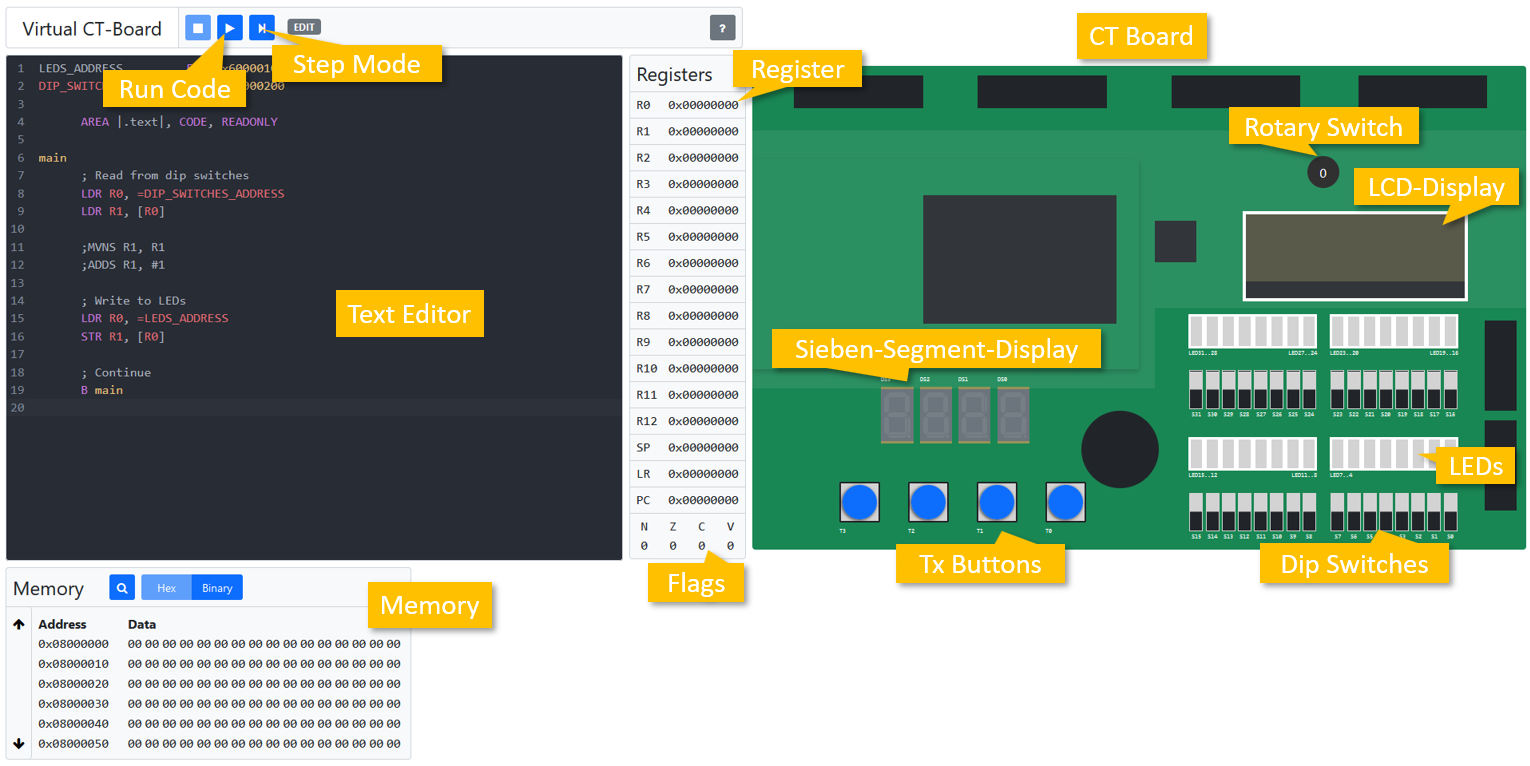
\includegraphics[width=\textwidth]{final}
\caption[size=8pt]{Die Grafikoberfläche des virtuellen CT Boards.}
\label{final}
\end{figure}

\subsection{Funktionen des \glqq Virtual CT Boards\grqq}

Der Ansatz des Entwicklungsteams bestand darin, die Komponenten des CT Boards gemäss der vermittelten Inhalte der CT1-Vorlesung so simpel wie möglich und so genau wie nötig nachzubauen.

\paragraph{Prozessor} Wie auch das physische CT Board verfügt das virtuelle Board über einen Prozessor samt \emph{Arithmetic Logic Unit} und Registern. Dieser bildet das Kernstück der Anwendung, denn dort finden die Ausführung des Programmcodes und die Berechnungen statt. 

\paragraph{Memory} Im Memory werden sämtliche Daten abgelegt: Dazu gehören die Programm-Instruktionen in Form des sogenannten Opcodes sowie die Daten, die durch die Inputfunktionen des Boards hereinkommen.

\paragraph{Input/Output} Folgende Komponenten stellen Input-Funktionen bereit: Die \emph{Dip Switches} und die Tx-Buttons als binäre On-/Off-Schalter und der \emph{Rotary Switch}, der kreisum gedreht werden kann. Als Output-Komponenten stehen die LED-Lämpchen, das Sieben-Segment-Display für die Darstellung vierstelliger Symbole und das LCD-Display für Text- und Farbanzeige zur Verfügung.

\paragraph{Assembler-Befehle} Alle für die CT1-Praktika relevanten Instruktionen der Assembler-Sprache wurden umgesetzt und sind im \glqq Virtual CT Board\grqq{} verwendbar. Dazu gehören:
\begin{itemize}
	\item[$-$] Datentransfer-Operationen: \emph{Move}, \emph{Load} und \emph{Store}
	\item[$-$] arithmetische Operationen: \emph{Add}, \emph{Subtract} und \emph{Multiply}
	\item[$-$] \emph{Logical} und \emph{Shift/rotate} Operationen
	\item[$-$] Vergleichsoperationen: \emph{Compare} und \emph{Test}
	\item[$-$] Stack-Operationen: \emph{Push} und \emph{Pop} %%% Wurden diese tatsächlich noch umgesetzt?
	\item[$-$] Kontrollstrukturen: \emph{Conditional} und \emph{Unconditional branches}
\end{itemize}

\paragraph{Debugging} Der Step-Modus erlaubt es, Schritt für Schritt durch den Programmcode zu gehen und jede Zeile einzeln auszuführen.

\subsection{Ausführbare Praktika}

%%% Welche Praktika sind ausführbar? Sind überhaupt welche ausführbar?

Die manuellen Tests haben ergeben, dass von den insgesamt 11 Praktika xx ausführbar sind. Die Tabelle \ref{praktika} zeigt den Lauffähigkeitsstatus jedes Praktikums und listet bei jenen, die noch nicht ausführbar sind, die fehlenden Funktionen auf.

\rowcolors{2}{gray!10}{gray!40}
\begin{table}[ht]
\begin{tabular}{ | l | c | c |}
	\hline
    \textbf{Praktikum} & \textbf{Lauffähigkeit} & \textbf{Fehlende Funktion} \\
	\hline
    1 Target System & Nein & C Code \\
	\hline
    2 Bit Manipulations & Nein & C Code \\
\hline
    3 Introduction to Assembly & ??? & - \\
\hline
    4 Data Transfer Commands & ??? & - \\
\hline
    5 Arithmetic Operations & ??? & - \\
\hline
    6 Control Structure & ??? & - \\
\hline
    7 Structured Programming in Assembly & ??? & - \\
\hline
    8 Subroutines and Parameter Passing & Nein & Potentiometer \\
\hline
    9 Linker & Nein & C Code \\
\hline
    10 Multiplication & ??? & - \\
\hline
    11 Interrupt & Nein & Interrupts \\
\hline
\end{tabular}
\caption[size=8pt]{Lauffähigkeitsstatus aller Praktika des CT1-Moduls auf dem virtuellen CT Board.}
\label{praktika}
\end{table}

\section{Diskussion und Ausblick}

Die aktuelle Version der Software ermöglicht es, einige der Praktika des CT1-Moduls virtuell durchzuführen. Damit ist der Grundstein für die Ersetzung der physischen CT Boards gelegt. Die Studierenden können nach und nach auf das \glqq Virtual CT Board\grqq{} umsteigen - wenn auch noch nicht vollständig. Bis alle Praktika von CT1 auf dem \glqq Virtual CT Board\grqq{} lauffähig sind, könnten im CT1-Unterricht die physischen Boards neben dem virtuellen eingesetzt und damit die bestehenden Ressourcen ideal ausgeschöpft werden. Falls die ZHAW Interesse daran hat, das \glqq Virtual CT Board\grqq{} weiter zu entwickeln und auch finanziell zu unterstützen, bietet sich die Umsetzung folgender Punkte an, für die die aufgewendete Zeit im Rahmen des PM4-Moduls nicht ausgereicht hat:

\begin{itemize}
	\item[$-$] Einige Assembler-Funktionen und Befehle wurden noch nicht umgesetzt, insbesondere die Interrupts, die in späteren CT1-Praktika behandelt werden, aber auch kleinere Befehle wie die \emph{Extend-} und \emph{Reverse-}Operationen.
	\item[$-$] Für die ersten beiden Praktika sowie Praktikum 9 müsste auch C-Code interpretier- und ausführbar sein.
	\item[$-$] Idealerweise sollte die Applikation das Laden und Speichern von Assembler-Files ermöglichen, damit die Studierenden ihre Arbeit jederzeit sichern und fortsetzen können.
	\item[$-$] Um auch komplexere Praktika durchführbar zu machen, muss der Text Editor mehrere Assembler-Files laden, anzeigen und ausführen können.

%%% Allenfalls Weiteres

\end{itemize}


Sollte die ZHAW zudem eine Erweiterung der Software anstreben, könnten zukünftig auch folgende Funktionalitäten umgesetzt werden: 
\begin{itemize}
\item[$-$] Implementierung einer vorbereiteten Bibliothek aller Praktika und Übungen des Moduls \glqq Computertechnik 1\grqq. 
\item[$-$] Implementierung der Funktionalitäten, welche für das Modul \glqq Computertechnik 2\grqq{} vorausgesetzt sind. 
\item[$-$] Implementierung einer virtuellen Darstellung von Signalen auf einem Oszilloskop.
\end{itemize}

\section{Literaturverzeichnis}

\begin{itemize}

\item[$-$] \emph{https://ennis.zhaw.ch} [abgerufen am 30.03.2022]
\item[$-$] \emph{https://salmanarif.bitbucket.io/visual/index.html}. [abgerufen am 30.03.2022]
\item[$-$] West, Steve (2018). Meeting Millennial Expectations In These Four Areas Of Technology. \emph{https://www.forbes.com/sites/forbestechcouncil/2018/06/28/meeting-millennial-expectations-in-these-four-areas-of-technology/?sh=5df2822f4ffc} [Abgerufen am 25.04.2022]
\item[$-$] Wirthman, Lisa (2020). How Tech-Savvy Millennials Are Driving the Digital Workplace. \emph{https://www.dell.com/en-us/perspectives/how-tech-savvy-millennials-are-driving-the-digital-workplace/} [Abgerufen am 25.04.2022]

\end{itemize}



\end{document}